\newif\ifdraft\drafttrue  % set true to show comments
\newif\ifplentyoftime\plentyoftimefalse  % :-)

\documentclass{svproc}

\usepackage{amsmath, amssymb, verbatim, enumerate, graphicx, centernot, tikz,
  array, mathtools, bussproofs, stmaryrd, enumitem, stackengine, subcaption}
\captionsetup{compatibility=false}
\usepackage{relsize}
\usepackage{listings}
\lstset{
  language=Caml,
  basicstyle=\upshape\sffamily,
  keywordstyle=\upshape\sffamily\color{dkblue},
  keepspaces=true,
  framexleftmargin=1ex,
  framexrightmargin=1ex,
  showstringspaces=false,
  commentstyle=\itshape\rmfamily,
  columns=flexible,
  % BCP: I find this distracting:
  % stringstyle=\sffamily\color{dkred},
  mathescape
}
\newcommand{\cd}[1]{\lstinline[backgroundcolor=\color{white}]$#1$}


%%%%%
% Macros
% Colors
\definecolor{dkblue}{rgb}{0,0.1,0.5}
\definecolor{dkgreen}{rgb}{0,0.6,0}
\definecolor{dkred}{rgb}{0.6,0,0}
\definecolor{dkpurple}{rgb}{0.7,0,0.4}
\definecolor{olive}{rgb}{0.4, 0.4, 0.0}
\definecolor{teal}{rgb}{0.0,0.5,0.5}
\definecolor{orange}{rgb}{0.9,0.6,0.2}
\definecolor{lightyellow}{RGB}{255, 255, 179}
\definecolor{lightgreen}{RGB}{170, 255, 220}
\definecolor{teal}{RGB}{141,211,199}
\definecolor{darkbrown}{RGB}{121,37,0}

\newcommand{\FINISH}[3]{\ifdraft\textcolor{#1}{[#2: #3]}\fi}
\newcommand{\bcp}[1]{\FINISH{dkred}{B}{#1}}
\newcommand{\BCP}[1]{\FINISH{dkred}{B}{\bf #1}}
\newcommand{\afm}[1]{\FINISH{dkgreen}{A}{#1}}
\newcommand{\dpw}[1]{\FINISH{dkblue}{D}{#1}} % Toronto Maple Leafs Blue :-)
\newcommand{\saz}[1]{\FINISH{orange}{SZ}{#1}}
\newcommand{\ksf}[1]{\FINISH{teal}{K}{#1}}
\newcommand{\sam}[1]{\FINISH{dkpurple}{SM}{#1}}

% FOR Regular Expression names
\newcommand{\re}[1]{\ensuremath{\mathtt{#1}}}
\newcommand{\squash}[3]{\ensuremath{\mathit{squash} \; (#1, #2, #3)}}
\newcommand{\perm}[2]{\ensuremath{\mathit{perm}\; (#1)\; \mathit{with}\; #2}}
\newcommand{\normalize}[3]{\ensuremath{\mathit{normalize} \; (#1, #2, #3)}}
\newcommand{\sep}{\ensuremath{\; | \;}}
\newcommand{\canonizer}{\ensuremath{\mathit{Canonizer}}}
\newcommand{\bibtex}{\textsc{Bib}\TeX{}}
\newcommand{\get}{\ensuremath{\mathit{get}}}
\newcommand{\lput}{\ensuremath{\mathit{put}}}
\newcommand{\create}{\ensuremath{\mathit{create}}}
\newcommand{\eqrel}[1]{\ensuremath{\equiv_{#1}}}

\newcommand{\Name}{Optometrist}

\newcommand{\QRESize}{QS}
\newcommand{\CanonizerAndSpecSize}{CS}
\newcommand{\LensAndSpecSize}{LS}

\newcommand{\OpticianRuntime}{\textbf{OO}}
\newcommand{\SystemOnOptician}{\textbf{SO}}
\newcommand{\SystemOnBenchmarks}{\textbf{SS}}

%%%%%%%%%%%%%%%%%%%%%%%%%%%%%%%%%%%

\begin{document}
\mainmatter              % start of a contribution
%
\title{Synthesizing Quotient Lenses}
%
\titlerunning{Synthesizing Quotient Lenses}  % abbreviated title (for running
% head)                                     also used for the TOC unless
%                                     \toctitle is used
%
\author{}
%
\authorrunning{} % abbreviated author list (for running head)
%
%%%% list of authors for the TOC (use if author list has to be modified)
\tocauthor{}
%
\institute{}

\maketitle              % typeset the title of the contribution

\begin{abstract} 

{\em Lenses}~\cite{Lenses} specify bidirectional 
transformations between different data formats.  Writing a single lens
rather than two separate uni-directional transformations saves both
keystrokes and bugs, by reducing redundancy and by automatically
guaranteeing strong ``lens laws'' ensuring that the forward and backward
transformations interact well.  
%
{\em Quotient lenses}~\cite{quotientlenses} are a generalization of lenses
where each of the data formats is quotiented by some equivalence relation
and the lens laws are taken modulo equivalence.  This allows lenses to be
both simpler and more flexible, since whole equivalence classes of data
values can be handled all at once and inessential details like whitespace
and ordering of fields can be ignored.

\smallskip

However, while plain lenses are widely used in both standalone systems and
popular libraries, Boomerang~\cite{Boomerang} is the only implementation
currently offering quotient lenses.  One reason for this is that there is
some annoying redundancy in the quotient lens notation: The programmer must
separately specify (1) the data formats on each side of the lens, (2) the
equivalence relations over them, and (3) a lens between the canonical
representatives of the equivalence classes, even though, typically, these
three share a great deal of structure.  Moreover, writing the lens between
the equivalence classes can be challenging due to the rather fiddly, mainly
due to ``non-ambiguity'' conditions in the lens well-formedness rules.

\smallskip

In this paper, we address both of these issues.  First, we propose a novel
language of {\em Quotient Regular Expressions}, or QREs, which allows
programmers to specify a broad class of equivalence relations over regular
languages using a compact and convenient notation in which the regular
language and its equivalence classes are captured by a single expression.
We then define {\em QRE lenses}, a class of bijective quotient lenses that
are typed using QREs, and we show how to {\em synthesize} QRE lenses from their
QRE types and a set of input-output examples.  We demonstrate the
practicality of this approach by synthesizing QRE lenses between several
real-world data formats from the {\tt data.gov} database.
\end{abstract}

\section{Introduction}
A {\em lens} $\ell$ is a {\em bidirectional transformation} between a source
type $S$ and a target type $T$ in which the forward transformation
$\ell.\get$ and the backward transformation $\ell.\lput$ satisfy certain
round-tripping laws such as invertibility.

An example of a bidirectional transformation which we shall revisit
severally in this paper is a lens which converts citation records such as
\begin{verbatim}
@Book {conway,
  Author = "J. H. Conway",
  Title = {Regular Algebra and Finite Machines}
}
\end{verbatim}

\noindent stored in the \bibtex{} format to their equivalent representation 
\begin{verbatim}
%0 Book
%T Regular Algebra and Finite Machines
%A J. H. Conway
%F conway
\end{verbatim}

\noindent in the EndNote format, and vice versa.

Lenses have the advantage of saving the programmer from having to
write two seperate transformations rather than one. Also, lenses offer strong
guarantees about how the two transformations interact since lenses are
constrained by lens laws. 

However, these constraints are sometimes too strict. For example, a record in
the data may represented in many ways because of the presence of spurious
whitespace characters or because of the reordering of fields. Deriving a lens
which obeys the lens laws in such a case can be daunting and frustrating.

As a solution to this problem, Foster et al proposed {\em quotient lenses},
which are a generalization of lenses in which the source and target data are
considered modulo an equivalence relation. Quotient lenses are
both simpler and more flexible, since whole equivalence classes of data
values can be handled all at once and inessential details like whitespace
and ordering of fields can be ignored.

However many complicated equivalence relations are difficult to express in
Boomerang, the lens programming language in which Foster et al implemented
quotient lenses. For example, suppose that the \bibtex{} to EndNote
transformation is required to allow for whitespace to occur arbitrarily between
the words in the label, author and title fields as well as in between them, and
ignore the order in which the author and title fields occur in each record.
These rules allow for the \bibtex{} citations
\begin{verbatim}
    @Book {conway,
      Author = "J. H. Conway",
      Title = {Regular Algebra and Finite Machines},
    }
\end{verbatim}
and
\begin{verbatim}
    @Book{     conway,
        Title = {Regular Algebra 
                 and Finite Machines},
           Author = "J. H. Conway",     }
\end{verbatim}
to be considered the same, with the EndNote records having similar rules
defined on them.

While it is possible to express the equivalence on the \bibtex{} data above in
Boomerang, actually doing so is difficult. The difficulty arises from the fact
that the entire equivalence is composed of three separate equivalences which
nest and interact with each other in a way that makes them difficult to express
with the standard Boomerang combinators. Moreover, many of the equivalences
expressible in Boomerang require that the programmer first specify the data
itself in form of a regular expression before specifying the equivalence
relation on the data.

To address this issue, we propose the language of {\em Quotient Regular
Expressions} or QREs, which express a broad class of equivalence relations
directly on regular languages using a compact and convenient notation. For
example, with QREs we can specify \bibtex{} records as shown in
Figure~\ref{fig:example-qre}.

\begin{figure}[t]
\begin{lstlisting}
let wsp = [ \n\t\r]$^+$
let wsp_to_space = project wsp $\to$ " "
let valid_name = name | (name . wsp_to_space . (name . wsp_to_space)$^*$ . name)
let wsp_to_and = project (wsp . "and" . wsp) $\to$ " and "
let bib_names = valid_name | (valid_name . wsp_to_and . (valid_name . wsp_to_and)$^*$ . valid_name)
let bib_author = "author = \"" . bib_names . "\""
let title = word | (word . wsp_to_space . (word . wsp_to_space)$^*$ . word)
let bib_title = "title = {" . title . "}"
let bib_perm = perm (label, bib_author, bib_title) with (project ("," .wsp) $\to$ ",\n")
let bibtex = "@book{" . bib_perm . "}"
\end{lstlisting}
\caption{QRE specification of \bibtex{} records. }
  \label{fig:example-qre}
\end{figure}

The expression \cd{project [\n\t\r]}$^+$ $\to$ \cd{" "} is a QRE that matches any 
number of whitespace characters, and then considers all strings of whitespace
characters as equivalent with a single space as the canonical representative. 
Another QRE in the example above is the

\begin{center}
\begin{lstlisting}
perm (label, bib_author, bib_title) with (project ("," . wsp ) $\to$ ",\n")
\end{lstlisting}
\end{center}

\noindent QRE, which specifies that the label, title and author fields can occur
in any order, with the fields separated by a comma followed by arbitrary amounts
of whitespace. The canonical representation is that in which the label, author
and title fields occur in that order, separated by a comma followed a newline.
The \cd{perm} QRE allows for easy nesting of permutations. Similarly, it is easy
to specify any number of fields within the \cd{perm} QRE.

While QREs make it easier to write quotient lenses by specifying the data and
the equivalence relation on the data in one expression, the programmer still
has to manually derive the underlying lens which maps the equivalence classes
of the source data to the equivalence classes of the target data. This is
itself tedious and error-prone task, as the code snippet below illustrates:

\begin{lstlisting}
let preamble : (lens in "@book{" $\Leftrightarrow$ "%0 Book\n%F ") = 
    del "@book{" . ins "%0 Book\n%F "
  
let author_lens : (lens in (",\n" . bib_author) $\Leftrightarrow$ ("\n" . end_author)) = 
    del ",\nauthor = \""
    . ins "\n%A "
    . valid_name
    . (del " and "
         . ins "\n"
         . (ins "%A " . valid_name . del " and " . ins "\n")$^*$ . ins "%A "
         . valid_name
           || "")
           
let title_lens : (lens in ("\",\n" . bib_title . "},\n}") $\Leftrightarrow$ ("\n" . end_title)) =
   del "\",\ntitle = {" . ins "\n%T " . title . del "},\n}" 
    
let bib_to_end : (lens in bib_tex $\Leftrightarrow$ end_note) =
   preamble . label . author_lens . title_lens
\end{lstlisting}

This lens transforms the \bibtex{} data to the EndNote (and vice versa) data by
matching the delimiters and separators in a bijective manner. For example,
the \cd{preamble} lens replaces the \bibtex{} preamble \cd{@book} with the
EndNote preamble \cd{\%0 Book\n\%F } in the \bibtex{} record. The programmer
can ill afford to make a mistake with any one of the small but vital details
of the transformations since even a one character mistake might render the lens
incorrect. This makes lens programming tedious and error-prone.

Therefore, to address this challenge, we identify a special class of quotient
lenses which we call {\em QRE lenses}, and show how to {\em
synthesize} QRE lenses from a pair of QREs and a set of input-output
example pairs. Our key insight is to reduce the problem of synthesizing QRE
lenses to the problem of synthesizing {\em bijective lenses}, which are the
bijections created from the Boomerang lens combinators. This is a problem
which we solved in our prior work ~\cite{popl18}.

QRE lenses lenses are the same as bijective lenses with ``canonizers at the
edges'' as in Figure~\ref{fig:attheedges}, and are typed using QREs. In the
forward direction, a QRE lens $q$ uses the source QRE $c$ to compute a unique
representative for the data modulo the equivalence relation defined by $c$ and
then applies the $\get$ function of a bijective lens $\ell$ to this
representative. In the backward direction, $q$ operates similarly,  but using
the view QRE $c'$ and the $\lput$ function of $\ell$.

\begin{figure}[t]
  \centering
  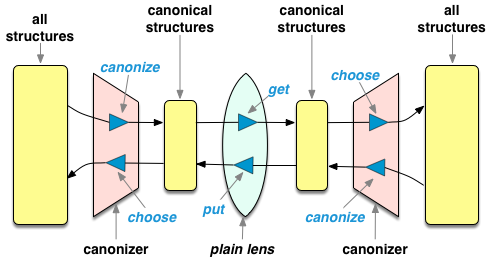
\includegraphics[width=\textwidth]{canonizers-outside}
  \caption{Quotient Lens with ``Canonizers at the Edges''\sam{This is a
      screenshot from Nate's thesis. Are we allowed to use it?}\bcp{We can
      (if we put ``from [Nate's thesis]'' in the caption), but I don't think
      we want the full complexity of asymmetric lenses here.  We should draw
      the figure again.  (I have the OmniGraffle file for it, so this is
      easy if I know how it should look.)}\bcp{Done---what do you think?}}
  \label{fig:attheedges}
\end{figure}

One potential pitfall with QRE lenses is that the combinators which
we define on them may not preserve this normal form. For example, the
composition $q' \circ q$ of QRE lenses $q$ and $q'$ may not be equivalent to
any quotient lens which has the canonical normal form of a bijective lens with
canonizers a the edges. Our main technical contribution in this paper is a
proof that QRE lenses are closed under left quotienting, right quotienting,
composition, and regular combinators.\bcp{If this is our main technical
  contribution, then it deserves more than a sentence in the intro!  E.g.,
  can we give an example?} This proof will allow justify our
approach for synthesizing quotient lenses so that the programmer can simply
type

\begin{lstlisting}
let bib_to_end : (lens in bibtex <=> endnote) 
= synth bibtex <=> endnote  using  {(bib_example, end_example)}
\end{lstlisting}
\noindent to synthesize a quotient lens that maps between \cd{bibtex} and
\cd{endnote} QREs, and sends the equivalence class of \cd{bib_bexample} to
the equivalence class of \cd{end_example}.

In summary, our main contributions are:
\begin{enumerate}
\item We introduce a novel language of {\em Quotient Regular Expressions}
(QREs) that provide compact, convenient notation for a natural and useful
class of equivalence relations on regular languages (Section~\ref{QRE}).
\item We define a language of {\em QRE lenses}, a subset of bijective quotient
lenses whose types are given by QREs.  Our main technical contribution is a
normal form for QRE lenses and a proof that normal forms are
closed under left quotienting, right quotienting, composition, and regular
operators (Section~\ref{QRE-lenses}).
\item Using this normal form, we reduce the problem of {\em synthesizing}
QRE lenses from their QRE types and a set of examples to the previously studied
problem of synthesizing bijective lenses between regular languages 
(Section~\ref{synth}).
\item We extend the Boomerang {\em implementation} with QREs, QRE lens operators,
and QRE lens synthesis and demonstrate its applicability by using it to
synthesize QRE lenses between several real-world data formats from the
{\tt data.gov} database (Section~\ref{impl}).
\end{enumerate}
Sections~\ref{relwork} and~\ref{concl} discuss related and future work.

\section{Quotient Regular Expressions}
\label{QRE}

This section introduces Quotient Regular Expressions or QREs. QREs are regular
expressions augmented with syntax that lets them simultaneously express an
equivalence relation on the language described by the regular expression.

\subsection{Overview}

We have already encountered the \cd{project R} $\to$ \cd{s} QRE
which sends all elements of the language described by the regular expression
$R$ to the canonical representative $s$, and the

\noindent \cd{perm (q_1, ..., q_n) with q} QRE which sends all permutations of
the QREs $q_1, \ldots, q_n$ separated by the QRE $q$ to the canonical
QRE $q_1 \cdot q \cdot \ldots \cdot q \cdot q_n$.

Now consider a variant of the \bibtex{} to EndNote example transformation,
where, the only quotienting occurs in the author field, where the author's name
can have the last name followed by a comma and then the rest of the name, or
remain as before where the names are separated by a space.

For example, these two records should be considered equivalent:
\begin{verbatim}
@Book {conway,
  Author = "Conway, J. H.",
  Title = {Regular Algebra and Finite Machines},
}
\end{verbatim}
\begin{verbatim}
@Book {conway,
  Author = "J. H. Conway",
  Title = {Regular Algebra and Finite Machines},
}
\end{verbatim}

The equivalence described is one in which there is a bijection between 
the regular expressions \cd{comma_name} and \cd{space_name} given by,
\begin{lstlisting}
let comma_name : regexp = name | (name . ", " . name . (" " . name)*)

let space_name : regexp = name | (name . " " . (name . wsp_to_space)* . name)

\end{lstlisting}

\noindent with the lens \cd{comma_to_space} mapping between them given by 
\begin{lstlisting}
let comma_to_space : (lens in space_name <=> comma_name) =
lens_swap 
(name . del " " . (ins " " . name . del " ")* ) (name . ins ", ") || name 
\end{lstlisting}

The $\squash{R}{R'}{f}$ QRE is designed to make it easy to express such
equivalences easily. Specifically, given regular expressions $R$ and $R'$, and
a function $f : \mathcal{L}(R) \longrightarrow \mathcal{L}(R')$, the
$\squash{R}{R'}{f}$ QRE expresses the equivalence relation on $\mathcal{L}(R \;
R')$ which sends each element $r \in \mathcal{L}(R)$ to the canonical element
$f(r) \in \mathcal{L}(R')$, and sends each element $r' \in \mathcal{L}(R')$ to
itself:

\begin{lstlisting}
let squash_author = squash space_name $\to$ comma_name using comma_to_space

let author : canonizer = "author = \"" . squash_author . "\""
\end{lstlisting}

In this example, the \cd{squash_author} QRE expresses the fact that the
\cd{space_name} and \cd{comma_name} representations of the authors' name
are equivalent, with the \cd{comma_name} representation chosen as the
canonical representation, and the lens \cd{comma_to_space} giving
the canonizing function which converts data in the \cd{space_name} format
to its \cd{comma_name} representation.

The $\squash{R}{R'}{\ell}$ has the added advantage that if the transformation
from $R$ to $R'$ can be expressed by a bijective lens that is consistent with a set
of examples, then the programmer can synthesize the lens from $R$ to $R'$
because of our previous work where we demonstrated how to synthesize bijective
lenses from a pair of regular expressions and a set of input-output example
pairs:

\begin{lstlisting}
let comma_to_space : (lens in space_name <=> comma_name) = 
synth space_name <=> comma_name using {("J. H. Conway", "Conway, J. H.")}
\end{lstlisting}

The regular combinators for QREs i.e. $\cdot$ (concatenation), $|$ (union) and
$*$ (iteration) behave like the regular combinators for regular languages. For
instance, if the QRE for matching a \bibtex{} record is named
\cd{bibtex}, then the QRE for matching two records is 
\cd{bibtex . bibtex}, the QRE for matching one or two records is
\cd{ bibtex | (bibtex . bibtex)} and the QRE for matching any number of QRE
records \cd{bibtex*}

The $\normalize{R}{R'}{f}$ expresses the equivalence relation which sends each
element in $\mathcal{L}(R)$ to its canonical representation $f(r) \in
\mathcal{L}(R')$. The equivalence relation defined by
$\normalize{R}{R'}{f}$ is thus the equivalence relation on
$\mathcal{L}(R)$ defined by the {\em fibres} of $f$ (i.e. $r \sim r'$ if and
only if $f(r) = f(r'))$. The canonizing function $f$ is required to be
surjective and idempotent.

The $\normalize{R}{R'}{f}$ QRE is the most general QRE in that for each QREs
$q$, there exist regular expressions $R, R'$ and a surjective, idempotent
function $f:\mathcal{L}(R) \longrightarrow \mathcal{L}(R')$ such that $q$ and
$\normalize{R}{R'}{f}$ each define the same equivalence relation on
$\mathcal{L}(R)$, with $\mathcal{L}(R')$ forming a complete set of
representatives for this equivalence relation. The $\normalize{R}{R'}{f}$
combinator is included so as to express equivalence relations which are
difficult to express, or which cannot be expressed, using the other
combinators. However, checking that the canonizing function $f$ is
surjective and idempotent is undecidable, thus we do not use the
$\normalize{R}{R'}{f}$ in practice. On the other hand, the
$\normalize{R}{R'}{f}$ combinator gives a sufficient condition for potential
QREs to be ``well-behaved'', particularly with respect to our strategy for
synthesizing quotient lenses which we shall introduce in Section~\ref{synth}.

While QREs express a broad class of equivalence relations on regular languages,
they do not express all the equivalence relations that can be expressed in
Boomerang, nor of course all the equivalence relations which cannot be
expressed using Boomerang canonizers. For instance, Boomerang canonizers can
map a regular language described by $R$ to a regular language described by
$S$, with $\mathcal{L}(S) \not \subseteq \mathcal{L}(R)$, whereas each QRE $q$
canonizes a regular language described by $R$ to regular subset
$\mathcal{L}(R') \subseteq \mathcal{L}(R)$ described by $R'$.

In summary each QRE $q$ enables us to express
\begin{enumerate}
  \item a regular expression $W(q)$ (the ``whole'' of $q$),
  \item an equivalence relation $\eqrel{q}$ on $\mathcal{L}(W(q))$,
  \item a regular expression $K(q)$ (the ``kernel'' of $q$)
  such that $\mathcal{L}(K(q))$ forms a complete set of representatives for
  $\eqrel{q}$, and
  \item a ``canonizing'' function $\canonizer(q):\mathcal{L}(W(q))
  \longrightarrow \mathcal{L}(K(q))$ which given any $w \in \mathcal{L}(W(q))$,
  computes $\canonizer(q)(w)$ as the unique $k$ in $\mathcal{L}(K(q))$ such that
  $k$ is equivalent to $w$ mod $\eqrel{q}$
  \end{enumerate}
  Observe that since $\canonizer(q)$ computes $\canonizer(q)(w)$ as the unique
  $k$ in $\mathcal{L}(K(q))$ such that $w$ is equivalent to $k$ mod $\eqrel{q}$,
  then the equivalence classes of $\eqrel{q}$ are the same as the fibres of
  $\canonizer(q)$.
\subsection{Syntax of QREs}
The language of Quotient Regular Expressions (QREs) is given by the following
grammar:
\begin{align*}
q := \; &R \sep R \mapsto s \sep \squash{R}{R'}{f} \sep
\perm{q_1, \ldots, q_n}{q} \;  | \; \normalize{R}{R'}{f}\\
&q' \circ q \sep q \cdot q' \sep (q \sep q') \sep q^*,
\end{align*}
where $R$ ranges over regular expressions, $f$ ranges over functions between
regular languages, and $s$ ranges over character strings.
  
\subsection{Semantics of QREs}
\subsubsection{Preliminaries}
Let $q, q'$ be QREs. When applying the regular combinators to QREs, we require
that if a string $s$ matches any of the regular expressions $W(q) \cdot W(q')$,
$W(q) \sep W(q')$, $W(q)^*$, $K(q) \cdot K(q')$,
$K(q) \sep K(q')$, $K(q)^*$, then $s$ matches that regular expression in
only one way. This unambiguity condition is called {\em strong unambiguity},
and is necessary, firstly because it ensures that the canonizing function of a
QRE is well-defined.

For example consider the QRE

\begin{lstlisting}
let ambiguous : canonizer = "a"* . (project "a"* $\to$ "a")
\end{lstlisting}

\noindent The behaviour of \cd{ambiguous} is not-well defined since the string
\cd{"aaa"} can be canonized to any of \cd{"a", "aa", "aaa"} depending on how
\cd{"aaa"} is parsed. We also require that the regular combinators applied to
the kernels are unambiguous since the underlying lenses will end up operating
on the kernels, and these lenses impose the same restrictions for similar
reasons.

To this end, we say that regular expressions $R$ and $S$ are
\textit{unambiguosly concatenable}, written $R \cdot^! S$ if for all strings
$r, r' \in \mathcal{L}(R)$ and $s, s' \in \mathcal{L}(S)$, if $r \cdot s = r'
\cdot s'$, then $r = r'$ and $s = s'$. We say that a regular expression $R$ is
\textit{unambiguosly iterable}, written $R^{*!}$ if for all strings $r_1,
\ldots, r_m$ and $r'_1, \ldots, r'_n \in \mathcal{L}(R)$, if $r_1 \cdot \ldots
\cdot r_m = r'_1 \cdot \ldots \cdot r'_n$, then $m = n$ and $r_i = r'_i$.

We say that a regular expression $R$ is \textit{strongly unambiguous} if and
only if (1) $R = \varnothing$, or (2) $R = S_1 \cdot S_2$ with $S_1, S_2$
strongly unambiguous and $S_1 \cdot^! S_n$, or (3) $R = S_1 \sep S_2$ with
$S_1, S_2$ strongly unambiguous and $\mathcal{L}(S_1) \cap \mathcal{L}(S_2) =
\varnothing$, or (4) $R = S^*$ with $S$ strongly unambiguous and $S^{*!}$.

The semantics for QREs that formally define the whole language $W(q)$, the
kernel language $K(q)$, the equivalence relation $\eqrel{q}$ and the
canonizing function $\canonizer(q)$ are given in
Figures~\ref{fig:wk},~\ref{fig:relations} and~\ref{fig:canonizers}.
\begin{figure}[t]
  \centering
  \[
    \begin{array}{l@{\quad}l@{\quad}l}
   
      q & W(q) & K(q) \\ \hline
      R & R & R \\
      R \mapsto s & W(q) & s \\
      \squash{R}{R'}{f} & R \sep R' & R' \\
      \normalize{R}{R'}{f} & R & R' \\
      q_1 \circ  q_2 & W(q_2) & K(q_1) \\
      q_1 \cdot q_2 & W(q_1) \cdot W(q_2) & K(q_1) \cdot K(q_2) \\
      q_1 \sep q_2 & W(q_1) \sep W(q_2) & K(q_1) \sep K(q_2) \\
      q^* & W(q)^* & K(q)^* \\
    \end{array}
  \]
\[
\begin{array}{r@{\quad}l}
W( \perm{q_1, \ldots, q_n}{q} ) = &
\bigcup \limits_{\sigma \in S_n} W(q_{\sigma(1)}) \cdot W(q) \cdot \ldots \cdot
W(q) \cdot W(q_{\sigma(n)})
\\
K( \perm{q_1, \ldots, q_n}{q} ) = &
 K(q_1) \cdot K(q) \cdot \ldots \cdot K(q) \cdot K(q_n) 
\end{array}
\]
  \caption{Whole and Kernel Regular Expressions\bcp{try putting the 
      last two clauses into the same format as the
      others (using $\mathit{qq} = ...$ and maybe reducing spacing around
      cdots, etc.)}}
  \label{fig:wk}
\end{figure}

\begin{figure}[t]
  \centering
\[
    \begin{array}{l@{\quad}l@{\quad}l} 
      w \; \equiv_R \; w' &\iff& w = w \\
      w \; \equiv_{R \mapsto s} \; w' \text{ for all }w, w'\\
      w \; \equiv_{\squash{R}{R'}{f}} \; w' &\iff& f(w) = w'
      \text{ or } w = w' \\
      w \; \equiv_{\normalize{R}{R'}{f}} \; w' &\iff&
      f(w)=f(w') \text{ or }w = w'\\
      w \; \equiv_{q_2 \circ q_1} \; w' &\iff& \exists k, k' \in
  \mathcal{L}(K(q_2)) \text{ such that } w \; \equiv_{q_1} \; k, \; w' \;
  \equiv_{q_1} \; k', \text{ and } k \; \equiv_{q_2} \; k'\\
      w \; \equiv_{q_1 \cdot q_2} \; w'  &\iff& w = r_1
      \cdot r_2, \; w' = {r'}_1 \cdot {r'}_2 \text{ with } r_1 \; \equiv_{q_1}
      \; {r'}_1, \; r_2 \; \equiv{q_n} \; {r'}_2\\
      w \; \equiv_{q' \sep q} \; w' &\iff& w \; \equiv_{q_1} \; w'
      \text{ or } \; w \; \equiv_{q_2} \; w'\\
      w \; \equiv_{q*} \; w' &\iff& w = r_1 \cdot \ldots \cdot r_n, \; w'
      = {r'}_1 \cdot \ldots \cdot {r'}_n \text{ and } r_i \equiv_{q} \; {r'}_i
      \\
      w \; \equiv_{\perm{q_1, \ldots, q_n}{q}} \; w' &\iff& w = r_{\sigma(1)}
      \cdot s_1 \cdot \ldots \cdot s_{n-1} \cdot r_{\sigma(n)}, \;
    w' = {r'}_{\theta(1)} \cdot s'_1 \cdot \ldots \cdot s'_{n-1}
    \cdot {r'}_{\theta(n)} \\
    & & \text{ for some } \sigma, \theta \in S_n, \text{ with } r_i \;
    \equiv_{q_i} \; r'_i \text{ and } s_k \; \equiv_{q} \; s'_{k}
    \end{array}
    \]
  \caption{QRE Equivalence Relations}
  \label{fig:relations}
\end{figure}
\begin{figure}[t]
  \begin{center}
\[
    \begin{array}{l@\quad l @\quad l} 
      \canonizer(R) &=& id_{\mathcal{L}(R)} \\
      \canonizer(R \mapsto s)(w) &=& s\\
      \canonizer(\squash{R}{R'}{f})(w) &=& 
\begin{cases}
f(w) & \text{if } w \in \mathcal{L}(R)\\
w & \text{otherwise}
\end{cases}\\
      \canonizer(\normalize{R}{R'}{f}) &=& f\\
      \canonizer(q' \circ q) &=& \canonizer(q') \circ \canonizer(q)\\
      \canonizer(q' \cdot q) &=& \canonizer(q') \cdot \canonizer(q)\\
      \canonizer(q_1 \sep q_2)(w) &=& 
\begin{cases}
\canonizer(q_1)(w) & \text{if } w \in \mathcal{L}(W(q_1))\\
\canonizer(q_2)(w) & \text{if } w \in \mathcal{L}(W(q_2))\\
\end{cases}\\
      \canonizer(q^*) &=& \canonizer(q)^* \\
    \end{array}
    \]
    \end{center}
    $\canonizer(\perm{q_1, \ldots, q_n}{q})(r_{\sigma(1)}
\cdot s_1 \cdot \ldots \cdot s_{n-1} \cdot r_{\sigma(n)}) \newline
= (\canonizer(q_1)(r_1)) \cdot (\canonizer(q)(s_1)) \cdot \ldots \cdot
(\canonizer(q_n)(r_n))$
  \caption{QRE canonizers}
  \label{fig:canonizers}
\end{figure}
\begin{figure}[t]
\centering
\begin{prooftree}
\AxiomC{$R$ is strongly unambiguous}
\UnaryInfC{$\mathit{id}(R)$ is well formed}
\end{prooftree}

\begin{prooftree}
\AxiomC{$s \in W(q)$}
\UnaryInfC{$R \mapsto s$ is well formed}
\end{prooftree}

\begin{prooftree}
\AxiomC{$\mathcal{L}(R) \cap \mathcal{L}(R') = \varnothing$}
\AxiomC{$f : \mathcal{L}(R) \longrightarrow \mathcal{L}(R')$}
\BinaryInfC{$squash(R, R', f)$ is well formed}
\end{prooftree}

\begin{prooftree}
\AxiomC{${\substack{\forall \sigma \neq \theta, \; W(q_{\sigma(1)}) \cdot W(q)
\cdot \ldots \cdot W(q_{\sigma(n)})\\ \cap W(q_{\theta(1)}) \cdot W(q)
\cdot \ldots \cdot W(q_{\theta(n)}) =\varnothing}}$}
\AxiomC{$q_i, q$ are well formed}
\AxiomC{$\forall \sigma, \; K(q_{\sigma(1)}) \cdot^! K(q) \cdot^! \ldots 
\cdot^! K(q_{\sigma(n)})$}
\TrinaryInfC{$\perm{q_1, \ldots, q_n}{q}$ is well formed}
\end{prooftree}

\begin{prooftree}
\AxiomC{$\mathcal{L}(R') \subseteq \mathcal{L}(R)$}
\AxiomC{$f : \mathcal{L}(R) \longrightarrow \mathcal{L}(R')$}
\AxiomC{$f$ is surjective}
\AxiomC{$f = f^2$}
\QuaternaryInfC{$normalize \; (R,R', f)$ is well formed}
\end{prooftree}

\begin{prooftree}
\AxiomC{$q$ is well formed}
\AxiomC{$q'$ is well formed}
\AxiomC{$K(q) = W(q')$}
\TrinaryInfC{$q' \circ q$ is well formed}
\end{prooftree}

\begin{prooftree}
\AxiomC{$q$ is well formed}
\AxiomC{$q'$ is well formed}
\AxiomC{$W(q) \cdot^! W(q')$}
\AxiomC{$K(q) \cdot^! K(q')$}
\QuaternaryInfC{$q \cdot q$ is well formed}
\end{prooftree}

\begin{prooftree}
\AxiomC{$q$ is well formed}
\AxiomC{$q'$ is well formed}
\AxiomC{$W(q) \cap W(q') = \varnothing$}
\TrinaryInfC{$q \cdot q$ is well formed}
\end{prooftree}

\begin{prooftree}
\AxiomC{$q$ is well formed}
\AxiomC{$W(q)^{*!}$}
\AxiomC{$K(q)^{*!}$}
\TrinaryInfC{$q^*$ is well formed}
\end{prooftree}
  \caption{QRE Inference Rules\bcp{Maybe some or all of these can be
      suppressed in the ``short version'' of the paper}\bcp{No, cancel
      that.  These are important.  And we need to comment about the decidability
    issues involving normalize.  (And a note that we don't really use
    normalize, but rather introduce more specialized instances.)}}
  \label{fig:qrerules}
\end{figure}
The theorem below confirms that the semantics of QREs are consistent with their
intended behaviour:
\begin{theorem}
If $q$ is a well formed QRE, then
\begin{enumerate}
  \item $W(q)$ and $K(q)$ are well defined regular expressions,
  \item  $\eqrel{q}$ is an equivalence relation on $\mathcal{L}(W(q))$,
  \item  $\mathcal{L}(K(q))$ forms a complete set of representatives for
  $\eqrel{q}$,
  \item $\canonizer(q):\mathcal{L}(W(q)) \longrightarrow \mathcal{L}(K(q))$ is a
  well-defined function, and
  \item  given any $w \in \mathcal{L}(W(q))$, $\canonizer(q)(w)$ is the unique
  $k$ in $\mathcal{L}(K(q))$ such that $k$ is equivalent to $w$ modulo
  $\eqrel{q}$.
  \end{enumerate}
\end{theorem}

\section{QRE Lenses}
\label{QRE-lenses} 
As we have seen, QREs express a broad class of equivalence relations
directly on regular languages.  QREs are therefore a good \textit{specification}
language for quotient lenses. In this section of the paper, we introduce
\textit{QRE Lenses}. QRE lenses are quotient lenses based on the Boomerang
quotient lens combinators, but which use QREs to describe their source and view
types.

Our approach in defining QRE lenses is as follows. Let $c, c'$ be QREs. Given a
bijection $\ell : K(c) \Leftrightarrow K(c')$, we may define a quotient lens $q
: W(c)/\eqrel{c} \Leftrightarrow W(c')/\eqrel{c'}$ by
\begin{equation}\label{normalform}
q.get = \ell \circ \canonizer(c) \text{ and } q.put = \ell^{-1} \circ
\canonizer(c'),
\end{equation}

\noindent One potential pitfall with QRE lenses is that the combinators which
we define on them may not preserve this normal form. For example, the
composition $q' \circ q$ of QRE lenses $q$ and $q'$ may not be equivalent to
any quotient lens which has the canonical normal form of a bijective lens with
canonizers a the edges. Consequently, in order to define quotient lenses, we
need to choose a class of bijections that has just the right properties with
respect to the quotient lens combinators. Our choice is to use the class of
\textit{bijective lenses}, a subset of the lenses expressible in Boomerang which
we identified and studied in our previous work~\cite{popl18}. Bijective lenses,
which we briefly discuss in the next subsection, possess the properties needed
to ensure that all QRE lenses have the normal form suggested in
\ref{normalform}.

\subsection{Bijective Lenses}
Define the set of \textit{bijective lenses} to be the set of bijections
between regular languages created from Boomerang lens combinators.
The syntax for the language of bijective lenses is given by
$$\ell := \mathit{id} \; (R) \sep const(s, s') \sep  swap(\ell,
\ell) \sep \ell \cdot \ell' \; |  \; (\ell \sep \ell') \sep \ell^* \;
| \; \ell \circ \ell',$$ where $R$ ranges over regular expressions and $s$
ranges over character strings.

‘The denotation of a lens $\ell$ is $\llbracket \ell \rrbracket \subseteq
\mathit{String} \times \mathit{String}$. If $(s_1, s_2) \in \llbracket \ell
\rrbracket$, then $\ell$ maps between $s_1$ and $s_2$.

\begin{align*}
\llbracket R \rrbracket &= \{(r, r) \sep r \in \mathcal{L}(R)\}\\
\llbracket swap(\ell, \ell') \rrbracket &= \{(s \cdot t, t' \cdot s') \sep
(s, s') \in \llbracket \ell \rrbracket \text{ and } (t, t') \in \llbracket
\ell' \rrbracket\}\\
\llbracket \ell \cdot \ell' \rrbracket &= \{(s \cdot t, s' \cdot t) \sep
(s, s') \in \llbracket \ell \rrbracket \text{ and } (t, t') \in \llbracket
\ell' \rrbracket\}\\
\llbracket \ell \sep \ell' \rrbracket &= \{(s \cdot t) \sep
(s, t) \in \llbracket \ell \rrbracket \text{ or } (s, t) \in \llbracket
\ell' \rrbracket\}\\
\llbracket \ell^* \rrbracket &= \{(s_1 \cdot \ldots \cdot s_n, t_1 \cdot \ldots
\cdot t_n) \sep (s_i, t_i) \in \llbracket \ell \rrbracket \text{ for } 1
\leq i \leq n\}
\end{align*}

The $\mathit{const}(s, t)$ lens replaces the string $s$ with $t$ in the source
data in the forward direction, and $t$ with $s$ in the view data in the backward
direction. $\mathit{id}(R)$ applies the identity function to the source and view
in $\mathcal{L}(R)$ in both directions. The composition lens $\ell' \circ \ell$
applies $\ell$ followed by then $\ell'$ to the source in the forward direction,
and applies $\ell'$ followed by $\ell$ to the view in the backward direction.
The lens $\ell \cdot \ell'$ first splits the string $s$ into $s_1$ and $s_2$,
applies $\ell$ and $\ell'$ to $s_1$ and $s_2$ to get $t_1$ and $t_2$
respectively, then concatenates $t_1$ and $t_2$ and returns $t_1 \cdot t_2$ as
the final result in the forward direction. $\ell \cdot \ell'$ operates
similarly in the backward direction, but with $s, s_1$ and $s_2$ substituted
for $t, t_1$ and $t_2$. The $\mathit{swap} \; (\ell, \ell')$ lens operates
like $\ell \cdot \ell'$, except that it swaps $t_1$ and $t_2$ before
concatenating the two for a final result of $t_2 \cdot t_1$ in the forward
direction. In the backward direction, $\mathit{swap}(\ell, \ell')$ first undoes
the swap, then proceeds as expected. The $\ell \; | \; \ell'$ lens
chooses to apply $\ell$ or $\ell'$ depending on whether the source
(resp. view) data is matched by $\ell$ or $\ell'$ in the forward (resp.
backward direction. The $\ell^*$ lens splits the string $s$ into strings $s_1,
\ldots, s_n$, applies $\ell$ to each $s_i$ to get $t_i$, and then concatenates
each of the $t_i$'s for a final result of $t_1 \cdot \ldots \cdot t_n$ in the
forward direction. $\ell^*$ operates similarly in the backward direction, but
with $s, s_i$ substituted for $t, t_i$.

Each bijective lens $\ell$ has a type $\ell : R \Leftrightarrow S$ where $R$ and
$S$ are regular expressions. If $\ell : R \Leftrightarrow S$, then the source
type of $\ell$ is $\mathcal{L}(R)$ and the view type of $\ell$ is
$\mathcal{L}(S)$. Interestingly, with the bijective lens type system, a lens
$\ell : R \Leftrightarrow S$ can also be considered to be of type $\ell : R'
\Leftrightarrow S'$ provided that $R$ (resp. $S$) can be proven to be
equivalent to $R'$ (resp. $S$) from the star-semiring axioms. The typing rules
for bijective lenses are given in Figure~\ref{fig:lensrules}. 

 \begin{figure}[t]
  \begin{prooftree}
\AxiomC{$s_1 \in \Sigma^*$}
\AxiomC{$s_2 \in \Sigma^*$}
\BinaryInfC{$\mathit{const} \; (s_1, s_t): s_1 \Leftrightarrow s_2$}
\end{prooftree}

\begin{prooftree}
\AxiomC{$R$ is strongly unambiguous}
\UnaryInfC{$\mathit{id} \; (R): R \Leftrightarrow R$}
\end{prooftree}

\begin{prooftree}
\AxiomC{$\ell_1 : R_1 \Leftrightarrow S_1$}
\AxiomC{$\ell_2 : R_2 \Leftrightarrow S_2$}
\AxiomC{$R_1 \cdot^! R_2$}
\AxiomC{$S_1 \cdot^! S_2$}
\QuaternaryInfC{$\ell_1 \cdot \ell_2: R_1 \cdot R_2 \Leftrightarrow S_1 \cdot
S_2$}
\end{prooftree}

\begin{prooftree}
\AxiomC{$\ell_1 : R_1 \Leftrightarrow R_2$}
\AxiomC{$\ell_2 : R_2 \Leftrightarrow R_3$}
\BinaryInfC{$\ell_2 \circ \ell_1: R_1 \Leftrightarrow R_3$}
\end{prooftree}

\begin{prooftree}
\AxiomC{$\ell_1 : R_1 \Leftrightarrow S_1$}
\AxiomC{$\ell_2 : R_2 \Leftrightarrow S_2$}
\AxiomC{$R_1 \cdot^! R_2$}
\AxiomC{$S_2 \cdot^! S_1$}
\QuaternaryInfC{$\mathit{swap} \; (\ell_1, \ell_2): R_1 \cdot R_2
\Leftrightarrow S_2 \cdot S_1$}
\end{prooftree}

\begin{prooftree}
\AxiomC{$\ell_1 : R_1 \Leftrightarrow S_1$}
\AxiomC{$\ell_2 : R_2 \Leftrightarrow S_2$}
\AxiomC{$\mathcal{L}(R_1) \cap \mathcal{L}(R_2) = \varnothing$}
\AxiomC{$\mathcal{L}(S_1) \cap \mathcal{L}(S_2) = \varnothing$}
\QuaternaryInfC{$\ell_1 \sep \ell_2: R_1 \sep R_2 \Leftrightarrow S_1 \sep S_2$}
\end{prooftree}

\begin{prooftree}
\AxiomC{$\ell : R \Leftrightarrow S$}
\AxiomC{$R^{*!}$}
\AxiomC{$S^{*!}$}
\TrinaryInfC{$\ell^*: R \Leftrightarrow S$}
\end{prooftree}

\begin{prooftree}
\AxiomC{$\ell : R \Leftrightarrow S$}
\AxiomC{$R \equiv R'$}
\AxiomC{$S \equiv S'$}
\TrinaryInfC{$\ell : R' \Leftrightarrow S'$}
\end{prooftree}
  \caption{Bijective Lens Typing Rules}
  \label{fig:lensrules}
\end{figure}

\subsection{Syntax of QRE Lenses}
Having given a brief overview of the class of bijective lenses, we now introduce
the class of QRE lenses, whose language is given by following grammar:
$$ q := \mathit{lift}(\ell) \sep \mathit{lquot}(q, \ell) \sep
\mathit{rquot}(\ell, q) \sep q \cdot q' \sep (q \sep q') \sep q^* \sep q \circ q',$$
where $\ell$ ranges over bijective lenses.

The QRE lens combinators are inspired by the Boomerang lens combinators of the
same name. The $\mathit{lift}(\ell)$ quotient lens enables a bijective lens
$\ell$ to be considered a quotient lens where the equivalence relation applied
to the source and view types is the equality relation, and the regular
combinators $\cdot \; * \; |$ on QRE lenses exhibit the expected behaviour,
with the caveat that the regular expressions used by these lenses are strongly
unambiguous.

The more interesting combinators are the $\mathit{lquot}$ and $\mathit{rquot}$
combinators. The $\mathit{lquot}(c, q)$ combinator takes a quotient lens $q$ and
quotients the source data using $c$, assuming that the source data forms a
complete set of representatives for the equivalence relation $\eqrel{c}$. The
$\mathit{lquot}(q, c)$ combinator does the same but on the view data. For
example, recall that in the \bibtex{} to EndNote transformation, we had the QREs
\cd{bibtex} and \cd{endnote} describing the \bibtex{} and EndNote records
respectively, and the bijective lens \cd{bib_to_end} that maps between
\cd{bibtex} and \cd{endnote}. The quotient lens which maps between
\cd{bibtex} and \cd{endnote} is given by the QRE lens

\begin{lstlisting}
let bib_to_end_q : (lens in bibtex <=> endnote) = 
rquot (lquot (bibtex, bib_to_end), endnote)
 \end{lstlisting} 
 
The difference between QRE lenses and Boomerang quotient lenses lies in the
typing judgements. More concretely, each QRE lens $q$ has a type $q : c
\Leftrightarrow c'$ where $c, c'$ are QREs. In contrast, the approach used to
type quotient lenses in Boomerang is to classify equivalences according to
whether they are or are not the equality relation. This type system is based on
two observations: first, that most quotient lenses originate as lifted basic
lenses, and therefore have types whose equivalence relations are both equality;
and second, that equality is preserved by many of the quotient lens
combinators. Foster et al also discuss a second possible approach to typing
quotient lenses, where equivalence relations are represented by rational
functions that induce them. While this second approach is more refined than the
first, Boomerang favours the first approach since the second appears to be too
expensive to be useful in practice~\cite{quotientlenses}.

\subsection{Semantics of QRE Lenses}
The denotation $\llbracket q \rrbracket$ of a QRE lens $q:c \Leftrightarrow c'$
is a quotient lens $\llbracket q \rrbracket : W(c)/{\eqrel{c}}
\Longleftrightarrow W(c')/{\eqrel{c'}}$. The typing rules and denotation of QRE
lenses are given in Figure~\ref{fig:qlenssemantics}. The following theorem
confirms that QRE lenses exhibit the intended behaviour.

\begin{theorem}
If there is a derivation $q:c \Leftrightarrow c'$ then
$\llbracket q \rrbracket : W(c)/{\eqrel{c}} \Leftrightarrow
W(c')/{\eqrel{c'}}$ is a well-defined quotient lens.
\end{theorem}

 \begin{figure}[t]
  \centering
  \begin{prooftree}
\AxiomC{$\ell : R \Leftrightarrow S$}
\UnaryInfC{$\mathit{lift}(\ell): R \Leftrightarrow id(S)$}
\end{prooftree}
  \begin{align*}
  \llbracket q \rrbracket.get &=  \llbracket \ell \rrbracket, \text{ and }\\
  \llbracket q \rrbracket.put &= \llbracket \ell \rrbracket^{-1}
  \end{align*}
 
\begin{prooftree}
\AxiomC{$q' : c'  \Leftrightarrow c''$}
\AxiomC{$c$ is well formed}
\AxiomC{$K(c) = W(c')$}
\TrinaryInfC{$\mathit{lquot}(c, q'): c' \circ c \Leftrightarrow c''$}
\end{prooftree}
  \begin{align*}
  \llbracket q \rrbracket.get  &= \llbracket q'
  \rrbracket.get \circ \canonizer(c)\\
  \llbracket q \rrbracket.put &= \llbracket q' \rrbracket.put
  \end{align*}

  \begin{prooftree}
  \AxiomC{$q' : c \Leftrightarrow c'$}
  \AxiomC{$c''$ is well formed}
  
\AxiomC{$K(c'') = W(c')$}
\TrinaryInfC{$\mathit{rquot}(q', c):c \Leftrightarrow c'' \circ c'$}
\end{prooftree}
  \begin{align*}
  \llbracket q \rrbracket.get &= \llbracket q'
  \rrbracket.get\\
  \llbracket q \rrbracket.put &= \llbracket q'
  \rrbracket.put \circ \canonizer(c'')
  \end{align*}
  
  \begin{prooftree}
\AxiomC{$q_1 : c \Leftrightarrow c'$}
\AxiomC{$q_2 : c' \Leftrightarrow c''$}
\BinaryInfC{$q_2 \circ q_1: c \Leftrightarrow c''$}
\end{prooftree}
  \begin{align*}
  \llbracket q \rrbracket.get &= \llbracket q_2 \rrbracket.get\circ \llbracket
  q_1 \rrbracket.get, \text{ and }\\
  \llbracket q \rrbracket.put &= \llbracket q_1 \rrbracket.put \circ \llbracket
  q_2 \rrbracket.put
  \end{align*}

    \begin{prooftree}
\AxiomC{$q' : c \Leftrightarrow c'$}
\AxiomC{$W(c)^{*!}$ and $W(c')^{*!}$}
\AxiomC{$K(c)^{*!}$ and $K(c')^{*!}$}
\TrinaryInfC{${q'}^* : c^* \Leftrightarrow {c'}^*$}
\end{prooftree}
  \begin{align*}
  \llbracket q \rrbracket.get &= (\llbracket q' \rrbracket.get)^*, \text{
  and }\\
  \llbracket q \rrbracket.put &= (\llbracket q' \rrbracket.put)^*
  \end{align*}

    \begin{prooftree}
\AxiomC{$q_1 : c_1 \Leftrightarrow d_1 $}
\AxiomC{$q_2 : c_2 \Leftrightarrow d_2$}
\AxiomC{${\substack{W(c_1) \cdot^! W(c_2)\\ K(c_1) \cdot^! K(c_2)}}$}
\AxiomC{${\substack{W(d_1) \cdot^! W(d_2)\\ K(d_1) \cdot^! K(d_2)}}$}
\QuaternaryInfC{$q_1 \cdot q_2: c_1 \cdot c_2
\Leftrightarrow d_1 \cdot d_2$}
\end{prooftree}
  \begin{align*}
  \llbracket q \rrbracket.get &= \llbracket q_1 \rrbracket.get \cdot \llbracket
  q_2 \rrbracket.get, \text{ and }\\
  \llbracket q \rrbracket.put &= \llbracket q_1 \rrbracket.put \cdot \llbracket
  q_2 \rrbracket.put
  \end{align*}

      \begin{prooftree}
\AxiomC{$q_1 : c_1 \Leftrightarrow d_1 $}
\AxiomC{$q_2 : c_2 \Leftrightarrow d_2$}
\AxiomC{$\mathcal{L}(W(c_1)) \cap \mathcal{L}(W(c_2)) = \varnothing$}
\AxiomC{$\mathcal{L}(W(d_1)) \cap \mathcal{L}(W(d_2)) = \varnothing$}
\QuaternaryInfC{$q_1 \sep q_2: (c_1 \sep c_2)
\Leftrightarrow (d_1 \sep d_2)$}
\end{prooftree}
  $$
  \llbracket q_1 \sep q_2 \rrbracket.get(s) = 
  \begin{cases}
  \llbracket q_1 \rrbracket.get (s) & \text{if } s \in \mathcal{L}(W(c_1))\\
  \llbracket q_2 \rrbracket.get (s) & \text{if } s \in \mathcal{L}(W(c_2))\\
  \end{cases}$$
  $$\llbracket q_1 \sep q_2 \rrbracket.put(s) = 
  \begin{cases}
  \llbracket q_1 \rrbracket.put (s) & \text{if } s \in \mathcal{L}(W(d_1))\\
  \llbracket q_2 \rrbracket.put (s) & \text{if } s \in \mathcal{L}(W(d_2))\\
  \end{cases}
  $$
  \caption{Denotation and Typing Rules for QRE Lenses\bcp{I think we can
      display this more compactly if we make the inference rules narrower by
    stacking the premises vertically and then put each inference rule {\em
      beside} its semantics definition.}}
  \label{fig:qlenssemantics}
\end{figure}

\subsection{Normal Forms of QRE Lenses}
Recall that our approach in defining QRE lenses is to have each QRE lens $q: c
\Leftrightarrow c'$ be such that 
\begin{align*}
\llbracket q \rrbracket.get &= \ell \circ \canonizer(c)\\
\llbracket q \rrbracket.put &= \ell^{-1} \circ
\canonizer(c')
\end{align*}
for some bijective lens $\ell$. We now provide a proof that all QRE lenses are
of this form.\bcp{Maybe some cases of the proof can be elided in the short
  version?} 
\begin{theorem}\label{normal form}
If there is a derivation $q : c \Leftrightarrow c'$, then there exists a
bijective lens $\ell : K(c) \Leftrightarrow K(c')$ such that
\begin{align*}
\llbracket q \rrbracket.get &= \llbracket \ell \rrbracket\circ \canonizer(c)\\
\llbracket q \rrbracket.put &= \llbracket \ell \rrbracket^{-1} \circ
\canonizer(c')
\end{align*}
\end{theorem}
\begin{proof}
Assume that $q : c \Leftrightarrow c'$. We proceed by induction over the
derivation $q : c \Leftrightarrow c'$.
\begin{enumerate}
  \item
  $\mathit{lift}(\ell): R/\mathit{id}(R) \Leftrightarrow S/\mathit{id}(S)$ where
  $\ell :
  R \Leftrightarrow S$. Then
  \begin{align*}
  \llbracket \mathit{lift}(\ell) \rrbracket.get &=  \llbracket \ell \rrbracket
  = \llbracket \ell \rrbracket \circ id_{\mathcal{L}(R)} =
  \llbracket \ell \rrbracket \circ \canonizer(\mathit{id}(R)), \text{ and }\\
  \llbracket \mathit{lift}(\ell) \rrbracket.put &= \llbracket \ell
  \rrbracket^{-1} = \llbracket \ell \rrbracket^{-1} \circ id_{\mathcal{L}(S)} =
  \llbracket \ell \rrbracket^{-1} \circ \canonizer(id(S))
  \end{align*}
  \item
  $\mathit{lquot}(c, q'): c' \circ c \Leftrightarrow c''$ where $q' : c' 
  \Leftrightarrow c''$, $c$ is well formed and $K(c) = W(c')$. Then
\begin{align*}
  \llbracket q \rrbracket.get  &= \llbracket q'
  \rrbracket.get \circ \canonizer(c)\\
  \llbracket q \rrbracket.put &= \llbracket q' \rrbracket.put
  \end{align*}
  By the induction hypothesis, there exists a bijective lens $\ell :
  K(c') \Leftrightarrow K(c'')$ such that 
  \begin{align*}
\llbracket q' \rrbracket.get &= \llbracket \ell \rrbracket \circ \canonizer(c')\\
\llbracket q' \rrbracket.put &= \llbracket \ell \rrbracket^{-1} \circ
Canonize(c'')
\end{align*}
Consequently
\begin{align*}
  \llbracket q \rrbracket.get  &= (\llbracket \ell \rrbracket \circ
  \canonizer(c')) \circ \canonizer(c) = \llbracket \ell \rrbracket \circ
  (\canonizer(c' \circ c))\\
  \llbracket q \rrbracket.put &= \llbracket \ell \rrbracket^{-1} \circ
  Canonize(c'')
  \end{align*}

  \item
  $\mathit{rquot}(q', c''):c \Leftrightarrow c'' \circ c'$ where $q' : c \Leftrightarrow
  c'$, $c''$ is well formed and $K(c'') = W(c')$. Proceed as in the previous
  case.
\item
$q_2 \circ q_1: c \Leftrightarrow c''$ where $q_1 : c \Leftrightarrow c'$ and
$q_2 : c' \Leftrightarrow c''$. Then
  \begin{align*}
  \llbracket q \rrbracket.get &= \llbracket q_2 \rrbracket.get\circ \llbracket
  q_1 \rrbracket.get, \text{ and }\\
  \llbracket q \rrbracket.put &= \llbracket q_1 \rrbracket.put \circ \llbracket
  q_2 \rrbracket.put
  \end{align*}
  By the induction hypothesis, there exist bijective lenses
  $\ell_1 :
  K(c) \Leftrightarrow K(c')$ and $\ell_2 : K(c') \Leftrightarrow K(c'')$ such
  that
  \begin{align*}
\llbracket q_1 \rrbracket.get &= \llbracket \ell_1 \rrbracket \circ
\canonizer(c)\\
\llbracket q_1 \rrbracket.put &= {\llbracket \ell_1 \rrbracket}^{-1} \circ
\canonizer(c')
\end{align*}
and
\begin{align*}
\llbracket q_2 \rrbracket.get &= \llbracket \ell_2 \rrbracket \circ
Canonize(c')\\
\llbracket q_2 \rrbracket.put &= {\llbracket \ell_2 \rrbracket}^{-1} \circ
Canonize(c'')
\end{align*}
Consequently,
\begin{align*}
\llbracket q_2 \rrbracket.get \circ \llbracket q_1 \rrbracket.get &=
(\llbracket \ell_2 \rrbracket \circ \canonizer(c')) \circ (\llbracket \ell_1
\rrbracket \circ \canonizer(c))\\
&= \llbracket \ell_2 \rrbracket \circ (\canonizer(c') \circ \llbracket \ell_1
\rrbracket) \circ \canonizer(c)\\
&= (\llbracket \ell_2 \rrbracket \circ \llbracket \ell_1 \rrbracket) \circ
\canonizer(c)\\
&= \llbracket \ell_2  \circ  \ell_1 \rrbracket \circ
\canonizer(c)
\end{align*} 
A similar argument shows that 
$$\llbracket q_1 \rrbracket.put \circ \llbracket q_2 \rrbracket.put =
\llbracket \ell_2  \circ  \ell_1 \rrbracket^{-1} \circ
\canonizer(c)$$
\item  
${q'}^* : c^* \Leftrightarrow {c'}^*$ where $q' : c \Leftrightarrow c'$,
$W(c)^{*!}$ and $W(c')^{*!}$ and $K(c)^{*!}$ and $K(c')^{*!}$. Then
  \begin{align*}
  \llbracket {q'}^* \rrbracket.get &= (\llbracket q' \rrbracket.get)^*, \text{
  and }\\
  \llbracket {q'}^* \rrbracket.put &= (\llbracket q' \rrbracket.put)^*
  \end{align*}
  By the induction hypothesis there exists a bijective lens $\ell : K(c)
  \Leftrightarrow K(c')$ such that 
   that
  \begin{align*}
\llbracket q' \rrbracket.get &= \llbracket \ell \rrbracket \circ
\canonizer(c)\\
\llbracket q' \rrbracket.put &= {\llbracket \ell \rrbracket}^{-1} \circ
\canonizer(c')
\end{align*}
Consequentlty
\begin{align*}
\llbracket {q'}^* \rrbracket.get &= (\llbracket \ell \rrbracket \circ
\canonizer(c))^* = \llbracket \ell \rrbracket^* \circ
\canonizer(c)^* = \llbracket \ell^* \rrbracket \circ
\canonizer(c^*)\\
\llbracket {q'}^* \rrbracket.put &= (\llbracket \ell \rrbracket^{-1} \circ
\canonizer(c'))^* = (\llbracket \ell \rrbracket^{-1})^* \circ
\canonizer(c')^* = \llbracket \ell^* \rrbracket^{-1} \circ
\canonizer(c'^*)\\
\end{align*}
\item
  $q_1 \cdot q_2: c_1 \cdot c_2 \Leftrightarrow d_1 \cdot d_2$, where $q_1 : c_1
  \Leftrightarrow d_1 $,  $q_2 : c_2 \Leftrightarrow d_2$, $W(c_1)
  \cdot^! W(c_2)$, $K(c_1) \cdot^! K(c_2)$, $W(d_1) \cdot^! W(d_2)$ and $
  K(d_1) \cdot^! K(d_2)$. Then
  \begin{align*}
  \llbracket q \rrbracket.get &= \llbracket q_1 \rrbracket.get \cdot \llbracket
  q_2 \rrbracket.get, \text{ and }\\
  \llbracket q \rrbracket.put &= \llbracket q_1 \rrbracket.put \cdot \llbracket
  q_2 \rrbracket.put
  \end{align*}
By the induction hypothesis, there exist bijective lenses $\ell_1 : K(c_1)
\Leftrightarrow K(d_1)$ and $\ell_2 : K(c_2) \Leftrightarrow K(d_2)$ such that
\begin{align*}
\llbracket q_1 \rrbracket.get &= \llbracket \ell_1 \rrbracket \circ
\canonizer(c_1)\\
\llbracket q_1 \rrbracket.put &= {\llbracket \ell_1 \rrbracket}^{-1} \circ
\canonizer(d_1)
\end{align*}
and
\begin{align*}
\llbracket q_2 \rrbracket.get &= \llbracket \ell_2 \rrbracket \circ
\canonizer(c_2)\\
\llbracket q_2 \rrbracket.put &= {\llbracket \ell_2 \rrbracket}^{-1} \circ
\canonizer(d_2)
\end{align*}
Consequently,
\begin{align*}
  \llbracket q \rrbracket.get &= (\llbracket \ell_1 \rrbracket \circ
\canonizer(c_1)) \cdot  (\llbracket \ell_2 \rrbracket \circ
\canonizer(c_2))\\
&= (\llbracket \ell_1 \rrbracket \cdot \llbracket \ell_2
\rrbracket) \circ (\canonizer(c_1) \cdot \canonizer(c_2))\\
&= \llbracket \ell_1 \cdot  \ell_2 \rrbracket \circ \canonizer(c_1 \cdot c_2)
\end{align*}
Similarly
$$
  \llbracket q \rrbracket.put = \llbracket \ell_1 \cdot  \ell_2 \rrbracket^{-1}
  \circ \canonizer(d_1 \cdot d_2) $$
  \item
  $q = q_1 \sep q_2$ where $q_1 : c_1 \Leftrightarrow d_1 $, $q_2 : c_2
  \Leftrightarrow d_2$, $\mathcal{L}(W(c_1)) \cap \mathcal{L}(W(c_2)) =
  \varnothing$ and $\mathcal{L}(W(d_1)) \cap \mathcal{L}(W(d_2)) = \varnothing$.
  Then
  $$
  \llbracket q_1 \sep q_2 \rrbracket.get(s) = 
  \begin{cases}
  \llbracket q_1 \rrbracket.get (s) & \text{if } s \in \mathcal{L}(W(c_1))\\
  \llbracket q_2 \rrbracket.get (s) & \text{if } s \in \mathcal{L}(W(c_2))\\
  \end{cases}$$
  $$\llbracket q_1 \sep q_2 \rrbracket.put(s) = 
  \begin{cases}
  \llbracket q_1 \rrbracket.put (s) & \text{if } s \in \mathcal{L}(W(d_1))\\
  \llbracket q_2 \rrbracket.put (s) & \text{if } s \in \mathcal{L}(W(d_2))\\
  \end{cases}
  $$
By the induction hypothesis, there exist bijective lenses $\ell_1 : K(c_1)
\Leftrightarrow K(d_1)$ and $\ell_2 : K(c_2) \Leftrightarrow K(d_2)$ such that
\begin{align*}
\llbracket q_1 \rrbracket.get &= \llbracket \ell_1 \rrbracket \circ
\canonizer(c_1)\\
\llbracket q_1 \rrbracket.put &= {\llbracket \ell_1 \rrbracket}^{-1} \circ
\canonizer(d_1)
\end{align*}
and
\begin{align*}
\llbracket q_2 \rrbracket.get &= \llbracket \ell_2 \rrbracket \circ
\canonizer(c_2)\\
\llbracket q_2 \rrbracket.put &= {\llbracket \ell_2 \rrbracket}^{-1} \circ
\canonizer(d_2)
\end{align*}
Consequently,
$$
  \llbracket q_1 \sep q_2 \rrbracket.get(s) = 
  \begin{cases}
  \llbracket \ell_1 \rrbracket \circ
\canonizer(c_1) (s) & \text{if } s \in \mathcal{L}(W(c_1))\\
  \llbracket \ell_2 \rrbracket \circ
\canonizer(c_2) (s) & \text{if } s \in \mathcal{L}(W(c_2)),\\
  \end{cases}$$
  so $\llbracket q_1 \sep q_2 \rrbracket.get = \llbracket \ell_1 \sep
  \ell_2 \rrbracket \circ \canonizer(c_1 \sep c_2)$. A similar argument shows
  that $\llbracket q_1 \sep q_2 \rrbracket.put = \llbracket \ell_1 \sep
  \ell_2 \rrbracket^{-1} \circ \canonizer(d_1 \sep d_2)$.\\
  This completes the proof.
\end{enumerate}
\end{proof}

\section{Synthesizing QRE Lenses}
\label{synth}
Our goal in this section is to demonstrate how to synthesize a quotient lens
$q: c \Leftrightarrow c'$ from the QREs $c, c'$ and a set of input-output pairs
$\{(x_1, y_1), \ldots, (x_n, y_n)\}$ where the $x_i$'s are in $W(c)$ and the
$y_i$'s are in $W(c')$.

We have shown in Theorem~\ref{normal form} that if there is a derivation $q : c
\Leftrightarrow c'$ of a QRE lens, then there exists a bijective lens $\ell :
K(c) \Leftrightarrow K(c')$ such that
\begin{align*}
\llbracket q \rrbracket.get &= \llbracket \ell \rrbracket\circ \canonizer(c)\\
\llbracket q \rrbracket.put &= \llbracket \ell \rrbracket^{-1} \circ
\canonizer(c')
\end{align*}

Now since the $x_i$'s are in $W(c)$ and the $y_i$'s are in $W(c')$, then

\noindent ${x_i}' = \canonizer(c)(x_i)$ is in $K(c)$ and ${y_i}' =
\canonizer(c')(y_i)$ is in $K(c')$, hence in order to synthesize the desired
quotient lens $q$ it suffices to synthesize a bijective lens $l : K(c)
\Leftrightarrow K(c')$ that is consistent with the canonized examples
$\{({x_1}', {y_1}'), \ldots, ({x_n}', {y_n}')\}$

In our previous work, we showed that given regular expressions $R, S$ and a set
of input-output pairs $\{(r_1, s_1), \ldots, (r_n, s_n)\}$, if there is a
derivation $\ell : R \Leftrightarrow S$ of a bijective lens that maps $r_i$ to
$s_i$ in the forward direction and $s_i$ to $r_i$ in the backward direction,
then there is an algorithm that computes a bijective lens $\ell' : R'
\Leftrightarrow S'$ such that $R \equiv R'$, $S \equiv S'$, $\ell'$ maps $r_i$
to $s_i$ in the forward direction and $s_i$ to $r_i$ in the backward direction,
and $\llbracket \ell \rrbracket = \llbracket \ell' \rrbracket$~\cite{popl18}.

This implies that if there is a derivation $q : c \Leftrightarrow
c'$ of a QRE lens as well as a derivation $\ell : K(c) \Leftrightarrow K(c')$
that is consistent with the canonized examples $\{({x_1}', {y_1}'),
\ldots, ({x_n}', {y_n}')\}$, then we can synthesize a quotient lens $q$ of
type $c \Leftrightarrow c'$ that is consistent with $\{({x_1}', {y_1}'),
\ldots, ({x_n}', {y_n}')\}$.

More specifically, in order to synthesize a quotient lens $q: c \Leftrightarrow
c'$, that is consistent with the examples $\{(x_1, y_1), \ldots, (x_n, y_n)\}$
 it suffices to perform the following procedure:
\begin{enumerate}
  \item
  Compute $K(c)$, $K(c')$,
  \item
  compute $\{({x_1}', {y_1}'), \ldots, ({x_n}', {y_n}')\}$ where ${x_i}' =
  \canonizer(c)(x_i)$ and ${y_i}' = \canonizer(c')(y_i)$,
  \item
    synthesize a bijective lens $\ell : K(c) \Leftrightarrow K(c')$ that is
    consistent with the examples $\{({x_1}', {y_1}'), \ldots, ({x_n}',
    {y_n}')\}$
  \item 
  return $q = \mathit{rquot}(\mathit{lquot}(c, \ell), c') : c \Leftrightarrow
  c'$
\end{enumerate}
As an example, recall that
in the \bibtex{} to EndNote transformation we had the QREs \cd{bibtex} and \cd{endnote} describing a \bibtex{} record and an
Endnote record respectively. We also had the example pair 
\cd{(bib_example , end_example)} where

\begin{lstlisting}
bib_example = 
"@Book {conway,
  Author = \"J. H. Conway\",
  Title = {Regular Algebra and Finite Machines},
}"
\end{lstlisting}

\noindent and

\begin{lstlisting}
end_example = 
"%0 Book
%T Regular Algebra and Finite Machines
%A J. H. Conway
%F conway"
\end{lstlisting}

Since the transformation between the kernel of \cd{bibtex} and the kernel of
\cd{endnote!} that maps \cd{bib_example!} to \cd{end_example} can be
expressed by a bijective lens, it suffices to type the expression

\begin{lstlisting}
let bib_to_end : (lens in bibtex <=> endnot) 
  = synth bibtex <=> endnote  using  {(bib_example, end_example)}
\end{lstlisting}

\section{Implementation and Evaluation}
\label{impl}


We have integrated QREs and quotient lens synthesis into Boomerang allowing QREs
and synthesis tasks to be expressed alongside existing Boomerang expressions.

All evaluations were performed on a 2.5 GHz Intel Core i7 processor with 16 GB
of 1600 MHz DDR3 running macOS High Sierra.

Our evaluations serve to answer the following questions:
\begin{enumerate}
\item Does synthesizing quotient lenses from QREs permit for an easier
  development process than existing approaches.

\item Are QREs sufficiently expressive that more lenses can be synthesized
  without modifications to the format. 

\item Is our synthesis algorithm competitive with existing lens synthesis
  tools.
\end{enumerate}

\subsection{Benchmark Suite Construction} 
Our benchmarks were constructed from two sources:
\begin{enumerate}
\item 39 of our benchmarks were derived from the Optician system.  These
  benchmarks were a combination of custom benchmarks, benchmarks derived from
  FlashFill, and benchmarks derived from Augeas.  Many of the formats mapped
  between had to be modified to work with the bijectivity constraints
  Optician required.  Commonly, one format had whitespace where the other did
  not allow for whitespace.  To address the bijectivity issues surrounding this,
  we added whitespace to the format that typically did not have whitespace.  We
  were able to remove these alterations in adopting these benchmarks to our
  system.

\item 8 of our benchmarks were derived from data.gov.  Data.gov contains
  many transformations between formats.  In addition to the formats previously
  adopted for Optician, we synthesized transformers between these formats.
\end{enumerate}

\subsection{Easing the Development Process}

To test if our tool eases the development process, we compare the following
number of AST nodes.
%
\begin{itemize}
\item[\QRESize{}] \QRESize{} is the number of AST nodes in the QRE
  specifications involved in QRE lens synthesis task.
\item[\CanonizerAndSpecSize{}] \CanonizerAndSpecSize{} is the number of
  AST nodes in $W(q)$ summed with the number of AST nodes in $\canonizer(q)$,
  for each QRE used in QRE lens synthesis task.
\item[\LensAndSpecSize{}] \LensAndSpecSize{} is the number of AST nodes
  in $W(q)$ summed with the number of AST nodes in the synthesized QRE lens.
\end{itemize}

The value of \QRESize{} represents the difficulty in writing our benchmarks.

The value of \CanonizerAndSpecSize{} represents the difficulty in writing our
benchmarks without QREs.  This is only an approximation, as both $W(q)$ and
$\canonizer(q)$ are automatically generated from the QRE.  In our
experience, these automatically generated regular expressions and canonizers are
the ones we would naturally write.

The value of \LensAndSpecSize{} represents the difficulty in writing our benchmarks
with neither QREs nor synthesis.  This is also an approximation, as $W(q)$ and
$\canonizer(q)$ and the bijective lens are all automatically generated.
We have found that the generated bijective lens is fairly similar in size to the
one we would manually write, though it is typically less modular.

Figure~\ref{?} shows the number of benchmarks written with at most a given
number of AST nodes.  We found that \QRESize{} was consistently smaller than
\CanonizerAndSpecSize{} and \LensAndSpecSize{}, demonstrating that introducing
QREs saves programmers programming effort compared to both Optician and basic
Boomerang.

\subsection{Increase of Expressivity}

Optician was only able to synthesize fully bijective data transformations.
\Name loosens that restriction, and is able to synthesize data which is
bijective when put in canonical form.
To determine the increase of expressivity, we analyzed:
\begin{enumerate}
\item How many data formats in Optician's benchmark suite required modifications
  to be bijective.
\item How many data formats in Optician's benchmark suite required modifications
  to be bijective when put in canonical form.
\end{enumerate}

We found that 10 of Opticians 39 benchmarks required modifications to be
bijective. We found that 4 of Optician's 39
benchmarks required modifications to be in bijective correspondence when in
canonical form.  Furthermore, we found that all of the data.gov examples
required no modifications to be in canonical form.  While we did not put the
data.gov examples into a form suitable for Optician, we found only 4 of
the 8 data.gov examples did not require canonization, so making suitable
for Optician would have required a modification of 4 of the data.gov
formats.

\subsection{Competitive Performance}

\begin{figure}
  \centering
  \begin{subfigure}[b]{.49\textwidth}
    \centering
    %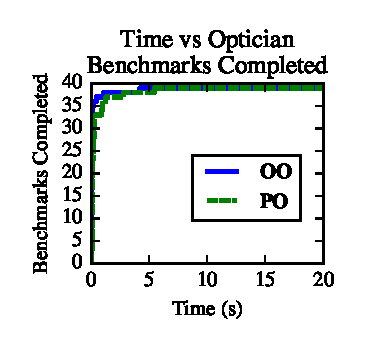
\includegraphics{generated-graphs/times_opt}
    \caption{}
    \label{subfig:lenssize}
  \end{subfigure}
  \begin{subfigure}[b]{.49\textwidth}
    %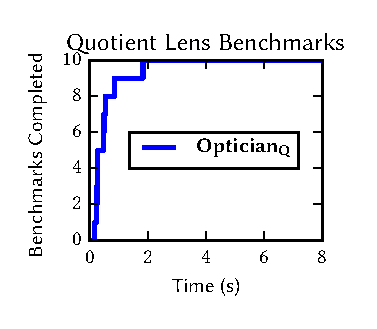
\includegraphics{times_new.eps}
    \caption{}
    \label{subfig:examplesused}
  \end{subfigure}
  \caption{Runtimes of Optician and \Name{}.
    In (a), we run Optician and \Name{} on Optician's benchmarks.  We find that
    there is only a negligible difference incurred by Optometrist's overhead.
    In (b), we run Optometrist on its benchmark suite.  We find that it is able
    to synthesize all quotient lenses in under 20 seconds, and typically
    finished in under 5 seconds. }
  \label{fig:times}
\end{figure}

While we expanded on the Optician system, we found it important to validate
performance did not degrade in this expansion.  To validate this, we tested:
\begin{itemize}
\item[\OpticianRuntime{}] Optician runs on its own benchmarks.
\item[\SystemOnOptician{}] \Name{} runs on Optician's benchmarks.
\item[\SystemOnBenchmarks{}] \Name{} runs on its own benchmarks.
\end{itemize}

We summarize the results of these experiments in Figure~\ref{fig:times}.
\Name{} was
able to synthesize all of Optician's benchmarks at a speed competitive with
Optician.  There was additional overhead in calculating $W(q)$ and $K(q)$,
resulting in a very slight decrease in performance.

Also notable was one of the data.gov examples, which converted demographic
statistics by zip code from xml form into rdf form.  This merely took longer because it was
an exceptionally large format, converting over 40 fields.  After adding in additional
fields to make this format bijective, it still took over 15 seconds to complete.

\section{Related Work}
\label{relwork} 

Bidirectional transformations have been used in diverse areas of computing
where they arise as parsers and pretty printers, marshallers
and unmarshallers, serializers and deserializers, database views and view
updaters and many others\sam{TODO put citations}. Such transformations have
been extensively studied since they were proposed as a solution to the classical
{\em view-update problem} in the database community, where the challenge is to
derive a program which extracts a view of data from a source, as well as a
program which folds view updates back into the source safely and correctly.

This paper builds on the work of Foster et al~\cite{quotientlenses} who
introduced the theory of quotient lenses and implemented quotient lenses as a
refinement of the bidirectional string processing language Boomerang.
In Boomerang, the source and target types are specified using regular
expressions, and the equivalence relations are expressed using canonizers, which
are functions that map elements of a regular language to their canonical
representative. Boomerang canonizers can express a very broad class of
equivalence relations between regular languages, but actually doing so is often
difficult with complicated equivalence relations. For instance, Boomerang's
in-build permutation combinator does not account for separators in between the
regular expressions. Also, this combinator permutes regular expressions rather
than canonizers, thus making it difficult to express nested permutations which
occur in many data formats, especially XML and XML-like formats.

In their paper, Foster et al also discuss other bidirectional programming
languages which support quotienting of data including XSugar~\cite{xsugar},
biXid~\cite{bixid} and X/Inv~\cite{xinv}. XSugar programs bidirectionally
convert data stored in XML and ASCII formats respectively, with the
transformations specified by a pair of unambiguous grammars. The quotienting
occurs on the XML side by use of a generic canonizer which standardizes the
representation of trees. Well-formed XSugar programs are guaranteed to be
bijective modulo an equivalence relation that captures XML normalization. biXid
programs convert between pairs of XML documents, with the XML formats specified
using a pair of grammars as in XSugar. However, biXid grammars can be ambiguous.
This ambiguity is what allows biXid to express equivalences on the data.
Finally, Foster et al discuss a possible connection with the language languages
X and Inv which support a primitive duplication combinator that does not work
well with the lens laws, but can be expressed using Boomerang quotient lenses.

As far as synthesis goes, though there is a good deal of recent research on
synthesizing unidirectional string
transformations~\cite{singh2012learning,le-pldi-2014,gulwani-popl-2014,
perelman2014test,Singh:blinkfill}, our system Optician, which we introduced in
~\cite{popl18}, is the first attempt to synthesize bidirectional
transformations that we are aware of. We compared Optician to two of these
unidirectional string transformers, Flash Fill~\cite{gulwani-popl-2014} and
FlashExtract~\cite{le-pldi-2014}, and found that these tools were unsuccessful
in synthesizing the complex transformations that can be expressed in Optician.
Furthermore, neither of these tools were able to infer transformations 
which occurred under two iterations.

Much of the research in synthesis assumes that the synthesizer is provided with
a collection of examples. Optician differs in that it requires that the
programmer supplies both examples {\em and} format descriptions in the form of
regular expressions. There are many other recent results showing how to
synthesize functions from type-based
specifications~\cite{augustsson-2004,osera+:pldi15,
feser-pldi-2015,scherer-icfp-2015,frankle+:popl16,armando+:pldi16}.
These systems enumerate programs of their target language, orienting their
search procedures to process only terms that are well-typed.
Optician is distinctive in that it synthesizes terms in a language with many
type equivalences. 
Perhaps the system most similar to Optician is InSynth~\cite{gvero-pldi-2013}, a
system for synthesizing terms in the simply-typed lambda calculus that addresses
equivalences on types.  

Morpheus~\cite{morpheus} is another synthesis system that uses two
communicating synthesizers to generate programs.  In both Morpheus and
Optician, one synthesizer provides an 
outline for the program, and the other fills in that outline with program
details that satisfy the user's specifications.
This approach works well in large search spaces, which
require some enumerative search.
One important way in which Optician differs from Morpheus is that in
Morpheus, an outline is a sketch---an
\emph{expression}
containing holes---whereas
an outline in Optician is a pair of regular
expressions, i.e., a 
\emph{type}.  Moreover, in order to implement an efficient
search procedure, we had to create both a new type language and a new
term language for lenses.  Once we did so, we proved our new, more
constrained language
designed for synthesis was just as expressive as the original, more
flexible and compositional language designed for human programmers.




\section{Conclusion and Future Work}
\label{concl}

\bcp{No bibliography??}

\end{document}
